\chapter{Introduction}
\label{sec:intro}

\section{Motivation and Problem Statement}

\subsection{Political Targets and Market Uptake of Electric Vehicles}

The transport sector accounts for a significant proportion of the UK total energy consumption and is to date mainly based on fossil fuels (\Autoref{fig:energy}). Across the EU personal and freight road transport cause 23\% of carbon emissions in equal shares \cite{Eurostat2017}. The steady rise in greenhouse gases, as well as dwindling reserves, are driving the link between the transport sector and an electricity sector that will be increasingly powered by renewable energy sources. Against the backdrop of climate change, the UK government has defined ambitious aspirations for decarbonising mobility and electricity supply following the EU's 2009 Renewable Energy Directive. By 2020, the UK aims to source 15\% of all energy and 10\% of transport fuels from renewables \cite{ECCC2016}. To date, however, only 4.23\% of transport fuels are supplied by sustainable energy including biofuels, whereas the electricity sub-target of 30\% by 2020 is projected to be surpassed by an additional 4\% \cite{ECCC2016}.

\begin{figure}[]
	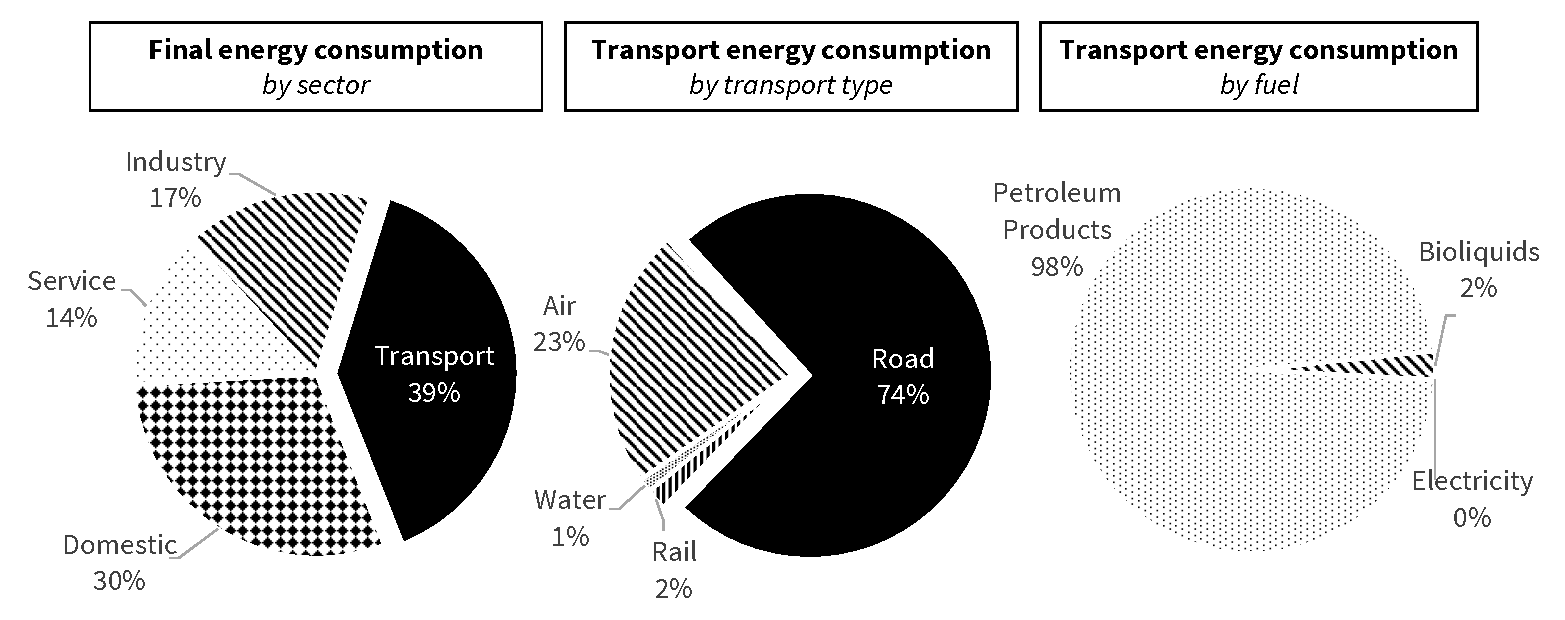
\includegraphics[width=\textwidth,trim={0cm 0cm 0cm 0cm},clip]{figures/energy.pdf}
	\caption{Final energy consumption of the UK by sector and fuel type for the year 2015 \cite{dfbei2017}}
	\label{fig:energy}
\end{figure}

The electrification of personal mobility is, nonetheless, a cornerstone of the UK's policy to reduce carbon emissions as well as air pollution in urban areas and is actively supported by government grant schemes and further incentives, which have overall been received favourably \cite{Knight2015}. The Plug-In Car Grant Scheme, operational since 2011, contributes a grant of 25\% but no more than \pounds 4,500 to the purchase cost of an eligible electric vehicle (EV). To date, more than 100,000 participants have made use of this incentive \cite{SMMT2017}. In 2013, the scheme was complemented with the Electric Vehicle Homecharge Scheme which reimburses costs for installing domestic charge points at home up to 75\%. Regional incentives such as the exemption from the London congestion charge add to the appeal of e-mobility.

Today, there are 87,000 electric vehicles on UK roads with new registrations peaking month to month \cite{ECCC2016}. While the market uptake is competitive compared to fellow European countries, electric vehicles yet only account for a marginal share of new car sales of approximately 2\% as of July 2017 \cite{SMMT2017}. However, recent news has nourished hope for progress. The car manufacturer Volvo pledged to exclusively produce electric vehicles from 2019 onwards \cite{Vaughan2017}. Tesla released its first long-range electric car Model 3 for the mass market, which has been praised for its affordability and excellent safety design \cite{Hern2017}. Most strikingly, in late July 2017 the UK government announced plans to ban all new petrol and diesel cars by 2040 in line with its previously published aspirations to have every new car powered by electricity by 2040 \cite{Knight2015}. By joining the Zero Emission Vehicle Alliance, the UK committed to a 100\% penetration rate of ultra low-emission vehicles (ULEV) in personal transport by 2050 \cite{ZeroEmissionVehicleAlliance2015}. Already for 2030, study \cite{Dof2008} predicts up to 20.6 million vehicles on UK roads in an extreme range scenario and at least 3 million under business as usual conditions.

\subsection{Challenges for Sustainable Electric Mobility}

% conditions
While the political will is a prerequisite, further conditions apply to achieve a sustainable transport sector. It must be untangled whether the transmission and distribution network capacity suffices to accommodate EV loads and how required supplemental renewable power can be integrated?

The additional load and rapid emergence of uncontrolled residential EV charging will negatively impact the low-voltage distribution network. The grid will be faced with an unprecedented energy demand, which had previously been supplied by diesel and petrol for ages. An average \mbox{3-person} household in the UK consumes \mbox{3,900 kWh} annually. With a consumption of \mbox{3,600 kWh}, an average EV with an annual mileage of \mbox{18,000 km} almost doubles overall electricity demand \cite{Knight2015}. Effects include excessive voltage drops, phase imbalances and overloading of network components, especially when many EVs charge simultaneously. Unfortunately, EV loads are likely to cluster when commuters arrive home at the end of the workday at similar times and plug-in their electric vehicles. Thus, immediate charging, especially in the evening at times of highest residual load, increases the detrimental impact. 

%% decarbonisation / renewable energy
Furthermore, a decarbonisation of electricity generation must accompany the expansion of electric vehicles since the specific CO$_2$-emissions of EVs depend largely on the composition of the generators that supply power at the time of charging current. Electric vehicles will only reveal their environmental supremacy over conventional vehicles if they are charged by renewable energy \cite{DLR2012}. Consequently, increased intermittent renewable energy generation will add to the need for smart grid management. Wind and photovoltaic power will take on an increasing share of electricity generation and are unable to follow electricity demand. Accordingly, there will be times when electricity demand is fully covered by renewable energy sources, but also those in which fossil fuels continue to dominate. For a safe power grid operation, demand and supply have to coincide exactly. Today it can be commonly observed that primarily wind turbines but also photovoltaic (PV) systems are shut down deliberately in order not to imperil grid stability in times of excess supply. For instance, the volume of unused energy by feed-in management trebled in 2014 compared to 2013 levels to 1.581 GWh in Germany as controllability on the supply side diminishes \cite{GermanysFederalNetworkAgency2016}.

\subsection{Solution Approaches for Sustainable Electric Mobility}

% Load flexibility / potential
Both aspects mandate increased levels of controllability on the demand side to reduce peak demand or match power supply; residential electricity demand becomes elastic. While investment in major network reinforcement is an intuitive measure to incorporate additional loads, it is deemed more economically efficient to encourage EV users to charge at off-peak times. Consensus exists that existing distribution networks can accommodate substantial penetration levels of electric vehicles if charging is coordinated. Exploiting typical load flexibility of parked electric vehicles by controlled charge scheduling as means of demand-side management will allow a mitigation of the network strains they evoke and can even provide a benefit to the grid integration of renewables \cite{Strbac2008}. This can be achieved by simple charge rate modulation with unidirectional power flow alone or additionally the provision of ancillary services with bidirectional power flow. Demand is fit to the current power supply by shifting loads under the umbrella of the renowned \textit{smart grid}, which \cite{Schuller2013} defines as the ``\textit{combination of enabling ICT \footnote{ICT = Information and Communication Technology} technologies that jointly make the power delivery infrastructure more reliable, versatile, secure and more accommodating for the integration of distributed and intermittent resources}''. Thereby, the electric vehicle unites aspects of an energy consumer and a regulation service provider simultaneously.

Traditionally, the network operators exercise balancing control using active and reactive power reserves offered by conventional generators and their costs are identified as intermittency costs of renewable energy generation, but under target-compliant market conditions controlled EV loads may intercept part of the demand and increase the resilience of power networks. Besides their load flexibility, electric vehicles are particularly suitable for demand side management for they can quickly respond to grid demand variation without startup or shutdown cost \cite{Han2011}. Moreover, EVs are already equipped with charge controllers and may implement profitable charging strategies \cite{Richardson2012}. \cite{Gottwalt2016} attests electric vehicles alongside stationary batteries and heat storages the most promising benefits for demand response.


%----------------------------
% Demand Side Management / Smart Grid / DR
%Definition of demand side management
%* all intentional electricity consumption pattern modifications by end-use customers, that are intended to alter the timing, level of instantaneous demand, or total electricity consumption
%Demand response (DR) can be defined as the changes in electricity usage by end-use customers from their normal consumption patterns in response to changes int he price of electricity over time or to incentive payments designded to induce lower electricity use at times of high wholesale market prices or when systems reliability is jeopardised (DoE2006, Albadi2008)
%Demand-Side Management (DSM) has traditionally been developed and centrally coordinated by utilities, often at the request of regulatory bodies seeking to minimize the operating cost base used to determine regulated tariffs for end users (Cooke2011)
% Dsm refers to classical, utility controlled meausres, while DR is the product of voluntary and independent decentralized decision-making by suppliers and customers.
%advantages \cite{Strbac2008}
%- reduction of generation reserves
%- capacity factor increase for available resources
%- reduction of emissions for power generation and balancing
%- improvement of transmission network efficiency
%- improvement of distribution network efficiency
%- improve the balancing of intermittent renewable energy sources
%- demand side elasticity in the power market
%Characteristics:
%- Low voltage grid
%- ICT to link and control devices
%- Decentral generation
%- Demand flexibility
%New Features:
%- Reliability: Due to using of Technologies for Fault-Detection
%- Efficiency: Due to Demand-Side Management
%- Load Balancing: Due to prediction algorithms for number of required generators
%- Sustainability: Due to renewable power sources
%--------------------------

% Financial Benefit
For users of electric vehicles to engage in coordinated charging and give up part of their flexibility, attractive monetary incentives, recharging reliability and low acceptance barriers are essential. Starting with simple night-time heating tariffs, time of use tariffs extend to more complex real-time pricing for price-responsive loads. Such dynamic tariffs based on day-ahead or intra-day spot markets are both, a reflection of the general network state and a source of cost minimisation potential for consumers. For the small-scale capacities of individual electric vehicles to gain access to large-scale wholesale electricity prices an intermediary is necessary to which multiple users surrender charging control. This so-called aggregator \textit{aggregates} sufficient demand and optimises electricity bill savings and revenue from the provision of regulation services by harnessing the load flexibility of the cars while observing network, equipment and demand constraints. Various organisational structures for aggregators are conceivable, but considering it as a subsidiary of the distribution network operator (DNO) reflects the technical responsibility for safe distribution network operation of the aggregator.

\begin{figure}[]
	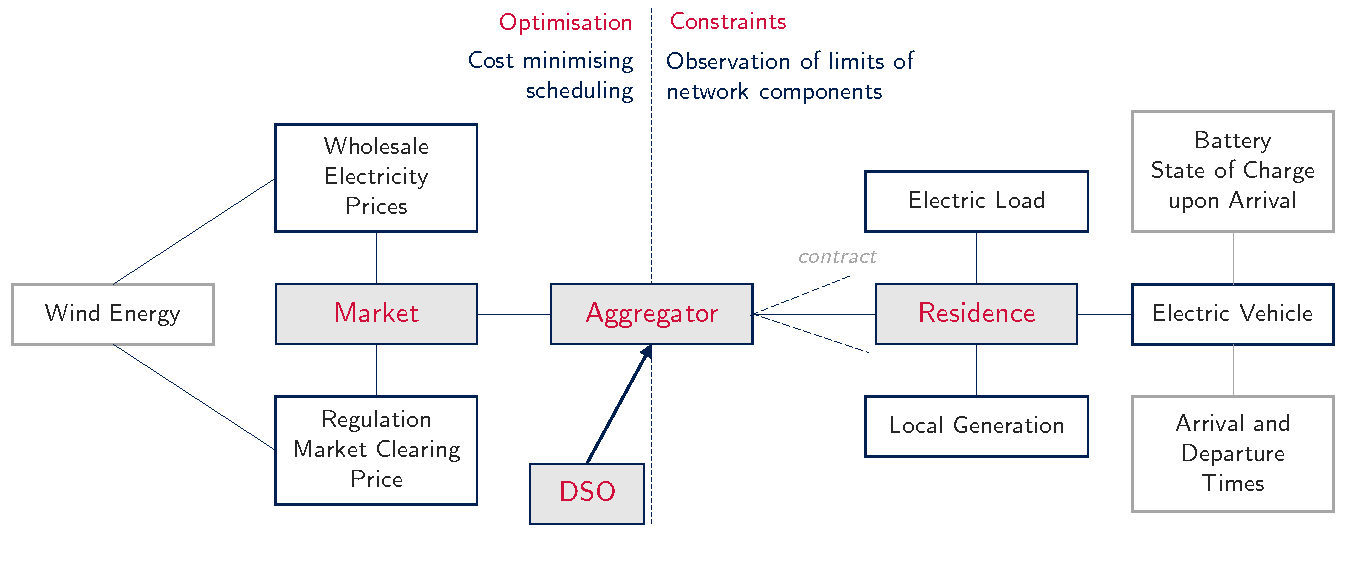
\includegraphics[width=0.9\textwidth,trim={0cm 0cm 0cm 0cm},clip]{figures/uncertainties/uncertainties.pdf}
	\caption{Overview of sources of uncertainty in EV scheduling}
	\label{fig:uncertainties}
\end{figure}

Day-ahead planning with the possibility to adapt charging schedules may be inevitable for market participation and finding the most efficient schedules. Meanwhile, the availability of electric vehicles is widely regarded as a key determinant of load shifting potential. While on an aggregate scale consumer behaviour is quite accurately predictable, forecasts on an individual level are prone to substantial deviations. A simple approach to circumvent this uncertainty is to enforce pre-set arrival/departure times by contractual obligations. Planning assumes fixed arrival and departure times. Even if the arrival times are stochastic, EV owners are often asked to specify their expected departure time and required battery charge to the aggregator for optimisation purposes \cite{Shi2011}. A relaxation of such constraints on users of electric vehicles could facilitate widespread adaptation of EV charging control, as besides preserving flexibility of use it omits inconvenient latency and diligence in communication. However, it also permits further uncertainty to the optimisation. To ensure a reliable battery charging processes, permitted uncertainty requires consideration by accurate prediction in conjunction with other, more inherent sources of uncertainty. As outlined in \Autoref{fig:uncertainties}, besides indeterminate arrival and departure times these are the battery charge levels on arrival, residential loads including the variability of local photovoltaic generation, and wholesale market prices influenced by the availability of large-scale renewable generators. Assessment of their impact on the performance of centralised charge control will be a principal contribution of this dissertation.

% other constraints / approaches
% -- Tesla power to provide link between local PV generation and EV charging -- investment? not everyone has PV but may use EV
%-- decentralised energy generation (PV), more independent power supply from the grid -- solution to both- more sustainable energy supply for EV demand and releasing local network strains

\subsection{Potential for Sustainable Electric Mobility}

% summary
In \cite{Daina2017} the preceding line of argument is shared and concisely summarised: ``\textit{On one hand electric grids capacity can be strained by an unmanaged EV load, especially at the distribution level where the capacity bottlenecks are most easily reached. On the other, if charging demand flexibility can be harnessed by implementing smart charging strategies, not only can costly grid capacity upgrades be minimised, but the operation of grid systems can be enhanced making use of a potentially very large responsive storage constituted by the batteries of grid-connected EVs.}''

% contribution
In short, electric vehicles can raise the share of renewable energy supply in a twofold manner if their charging processes are coordinated efficiently: first, they substitute fossil-fueled vehicles increasing the primary energy efficiency of the transport sector, and second, they facilitate the integration of renewable energy sources into the power grid via their load shifting capabilities.

\section{Research Questions and Objectives}
\label{sec:rq}

The primary goal of this dissertation is to develop a robust cost-minimising unidirectional day-ahead scheduling routine for charging electric vehicles overnight in residential low voltage distribution networks while observing local network, equipment and charging demand constraints in a stochastic environment under the participation in a wholesale electricity market. To build the stochastic environment in which residential electricity demand, market prices mirroring renewable energy supply and demand peaks, and the mobility behaviour of electric vehicle owners are uncertain, the secondary objective is to characterise and derive suitable models for inherent and conceded uncertainties incurred with the optimal scheduling of electric vehicles. Therefore, the contribution of this work is twofold: an \textit{optimisation study} complements the development of a stochastic \textit{simulation model}.

For the \textit{simulation model}, emphasis shall be put on investigating empirical uncertainty in the mobility behaviour of particular electric vehicle users to derive stochastic consumer behaviour about arrival and departure times as well as battery charge levels that not only addresses vagueness concerning the positioning of different user types but also uncertainty due to vehicle owners deviation from their predicted typical behaviour. This will facilitate the analysis of implications from relaxing commonly assumed contractual obligations for the consumers' EV availability and the aggregator's allocation of final battery state of charge. That is to assess how unexpected consumer behaviour limits the capability of a central scheduling entity to refill electric vehicle batteries.

The \textit{optimisation study} shall focus on the performance of multiple deterministic optimisation methods under uncertainty and approaches to mitigate the impact of individual prediction errors. It explores the possibility of attenuating the detrimental impact of uncertain parameters without the use of computationally complex stochastic programming techniques utilising critical information about parameter distributions and pre-specified degrees of conservatism. In addition to uniting consumer electricity bill savings with grid support through charge rate coordination, it aims to provide insight into the effectiveness and robustness of variants of analytical and heuristic approaches compared to na�ve reference optimisation methods, and the moderation between a customer's mobility requirements and cost savings. Furthermore, it should indicate financial benefits from participating in devised charging control schemes under today's and future market and tariff-design conditions to derive indicative policy recommendations for a frictionless transition to a sustainable electrified transport sector.

In summary, this work will address the following research questions:

\begin{enumerate}
	\item What are the major uncertainties involved in day-ahead scheduling of electric vehicles and how can they be modelled generically? In particular, how does limited knowledge on exact availability periods and battery charge levels limit the reliability of unaware scheduling approaches?
	\item How does the performance and robustness of analytical and heuristic scheduling methods compare despite uncertain inputs and how effective are proposed uncertainty mitigation options in reducing the number and severity of constraint violations?
	\item More accurately, what is the relative cost and benefit of increasing the robustness towards forecast deviations in day-ahead scheduling by applying increasing security margins to the deterministic optimisation approaches?
	\item How do tariff design and intra-day variance of prices affect the cost saving potential of devising charging control of electric vehicles to an aggregator with access to the wholesale electricity market?
\end{enumerate}

\newpage
\section{Dissertation Structure}

Having motivated the topic of electric vehicle scheduling and having defined the research questions of this work in \textbf{\Autoref{sec:intro}}, this dissertation consists of five further parts which are structured as follows:

\begin{itemize}
	\item \textbf{\Autoref{sec:found}} performs a literature review on previous approaches to electric vehicle charging coordination and categorises this work within the research field.
	\item \textbf{\Autoref{sec:model}} describes the simulation framework in which the EV scheduling is embedded and sequentially builds continuous models of required input parameters from empirical data including profound estimates of their uncertainties.
	\item In \textbf{\Autoref{sec:opt}} a deterministic optimisation problem for optimal EV scheduling in the stochastic environment is defined. It comprises an introduction to heuristic and analytical approaches implemented including simple reference optimisations and concludes with the introduction of multiple deterministic uncertainty mitigation concepts.
	\item In \textbf{\Autoref{sec:eval}} the configured optimisation methods and uncertainty mitigation approaches are evaluated in comparison to uncontrolled charging. Besides analysing resulting schedules, emphasis is put on the sensitivities of different degrees of conservatism in uncertainty mitigation and the impact of varying price spreads.
	\item \textbf{\Autoref{sec:concl}} provides a summary of results and answers obtained regarding the research questions, as well as an outlook on further research on the topic of EV scheduling.
\end{itemize}

